\documentclass[t,x11names,xcolor={x11names},hyperref={colorlinks,citecolor=Blue4,linkcolor=Blue4,anchorcolor=Blue4,urlcolor=Blue4}]{beamer}

% Neil: why discover races, because rare schedules often happen under load!

\setbeamertemplate{navigation symbols}{}
\useinnertheme{circles}
% \usecolortheme{crane}

% \usepackage[T1]{fontenc}
\usepackage[utf8]{inputenc}
% \usepackage[polish]{babel}
\usepackage[british]{babel}

% \usepackage[adobe-utopia]{mathdesign}
% \usepackage[series=z]{libgreek}
% \usepackage{tgpagella}
\usepackage[textwidth=4cm]{todonotes}
\usepackage{minted}
\usepackage{tcolorbox}
\tcbset{colframe=white,colback=white}
\usemintedstyle{colorful}
\usetikzlibrary{matrix,arrows,calc}
\def\diag{>=angle 60,thick}
\tikzset{every scope/.style={>=angle 60,thick}}

\author{Marcin Szamotulski}
\institute{
  \insertlogo{
\includegraphics[height=1cm]{iohk-logo.png}}\\
  
\includegraphics[width=2cm]{iohk.io.png}\\
}
\title{IOSim and Partial Order Reduction\\[5pt]}

\setbeamertemplate{frametitle}[default][center]
\setbeameroption{hide notes}

\begin{document}
\begin{frame}
    \titlepage
\end{frame}

\begin{frame}
  \frametitle{What is \href{https://hackage.haskell.org/package/io-sim}{IOSim}?}
  \href{https://hackage.haskell.org/package/io-sim}{\texttt{IOSim}} is a simulator monad that supports:
  \begin{itemize}
    \item asynchronous exceptions (including masking)
    \item simulated time
    \item timeout API
    \item software transaction memory (STM)
    \item concurrency: both low-level \texttt{forkIO} as well as \texttt{async} style
    \item strict STM
    \item access to lazy ST
    \item \textbf{schedule discovery}
    \item event log
    \item dynamic tracing
    \item tracing committed changes to \texttt{TVar}, \texttt{TMVar}s, etc.
    \item labeling of threads, \texttt{TVar}'s, etc.
  \end{itemize}
\end{frame}

\begin{frame}[fragile]
  \frametitle{\href{https://hackage.haskell.org/package/io-clases}{io-classes}}
  io-classes provide class based monad polymorphic api which allows to write
  code which can be executed both in \texttt{IO} and \texttt{IOSim}.\\

  \begin{minted}{haskell}
withAsyncs :: MonadAsync m
           => [m a]
           -> ([Async m a] -> m b)
           -> m b
withAsyncs xs0 action = go [] xs0
  where
    go as []     = action (reverse as)
    go as (x:xs) = withAsync x (\a -> go (a:as) xs)
  \end{minted}

  \vspace{1em}
  We also developed a few extensions which are packaged as a seprate libraries:
  \href{https://hackage.haskell.org/package/strict-stm}{strict-stm},
  \href{https://hackage.haskell.org/package/strict-mvar}{strict-mvar},
  \href{https://hackage.haskell.org/package/si-timers}{si-timers}.
\end{frame}

\begin{frame}[fragile]
  \frametitle{IOSim - trace}
  {\scriptsize
  \begin{minted}{haskell}
sim :: (MonadLabelledSTM m,
        MonadTimer m,
        MonadTraceSTM m,
        MonadSay m) => m ()
sim = do
    d <- registerDelay 1_000_000
    labelTVarIO d "delayVar"
    traceTVarIO d (\_ a -> pure (TraceString (show a)))
    atomically (readTVar d >>= check)
    say "Arr, land ho!"
  \end{minted}
  }

  {\tiny
  \begin{onlyenv}<2->
  \begin{verbatim}
0s - Thread []     main - RegisterDelayCreated TimeoutId 0 TVarId 0 Time 1s
0s - Thread []     main - TxBlocked [Labelled TVarId 0 delayVar]
0s - Thread []     main - Deschedule Blocked BlockedOnSTM
  \end{verbatim}
  \end{onlyenv}
  \begin{onlyenv}<3->
  \begin{verbatim}
1s - Thread [-1]   register delay timer - Say True
1s - Thread [-1]   register delay timer - RegisterDelayFired TimeoutId 0
  \end{verbatim}
  \end{onlyenv}
  \begin{onlyenv}<4->
  \begin{verbatim}
1s - Thread []     main - TxWakeup [Labelled TVarId 0 delayVar]
1s - Thread []     main - TxCommitted [] []
1s - Thread []     main - Unblocked []
1s - Thread []     main - Deschedule Yield
1s - Thread []     main - Say Arr, land ho!
1s - Thread []     main - ThreadFinished
1s - Thread []     main - MainReturn () []
  \end{verbatim}
  \end{onlyenv}
 }

\end{frame}

\note{
  Relation between Time and IOSimPOR.
}

\begin{frame}
  \frametitle{Partial Order Reduction}

  \begin{itemize}
    \item segment execution into execution steps, e.g. an \texttt{STM} action
    \item deterministic scheduling policy
    \item discovery of execution races which depends on execution steps partial
          order
    \item techniques to only run executions which can lead to new program
          states
    \item instrumentation to follow discovered schedules
  \end{itemize}
\end{frame}

\begin{frame}[fragile]
  \frametitle{Execution Step}
  \begin{minted}{haskell}
data Step = Step {
    stepThreadId :: IOSimThreadId,
    stepStep     :: Int,
    stepEffect   :: Effect,
    -- ^ which effects where executed by this steps, e.g.
    -- `TVar` reads / writes, forks, throws or wakeups.
    stepVClock   :: VectorClock
    -- ^ vector clock of the thread at the time when
    -- the step was executed.
  }
  deriving Show
  \end{minted}

  \texttt{IOSimPOR} thread scheduler will run one thread at a time, and collect
  \texttt{Step} for the period while the thread is being executed.
\end{frame}

\begin{frame}
  \frametitle{Execution Step}
  \framesubtitle{Life cycle of a \texttt{Step}}
  \begin{itemize}
    \item when a thread is descheduled:
      \begin{itemize}
        \item forking a new thread
        \item thread termination
        \item setting the masking state to interruptible
        \item popping masking frame (which resets masking state)
        \item thread delays
        \item execution of an STM transaction
        \item blocking \texttt{throwTo}
      \end{itemize}
    \item throw an exception when there's a corresponding catch frame (i.e. catch handler)
  \end{itemize}
\end{frame}

\begin{frame}[fragile]
  \frametitle{Execution Step}
  \framesubtitle{Effect}
  \scriptsize
  \begin{onlyenv}<1->
    \begin{minted}{haskell}
data Effect = Effect {
    effectReads  :: Set TVarId,
    effectWrites :: Set TVarId,
    effectForks  :: Set IOSimThreadId,
    effectThrows :: [IOSimThreadId],
    effectWakeup :: Set IOSimThreadId
  }
    \end{minted}
  \end{onlyenv}
  \begin{onlyenv}<2->
    \begin{minted}{haskell}
racingEffects :: Effect -> Effect -> Bool
racingEffects e e' =
       -- both effects throw to the same threads
       effectThrows e `intersects` effectThrows e'
       -- concurrent reads & writes of the same TVars
    || effectReads  e `intersects`  effectWrites e'
    || effectWrites e `intersects`  effectReads  e'
       -- concurrent writes to the same TVars
    || effectWrites e `intersects`  effectWrites e'
  where
    intersects :: (Foldable f, Eq a) => f a -> f a -> Bool
    intersects a b = not . null $ toList a `List.intersect` toList b
    \end{minted}
  \end{onlyenv}
\end{frame}

\begin{frame}[fragile]
  \frametitle{Execution Step}
  \framesubtitle{Causality}
  \begin{center}
  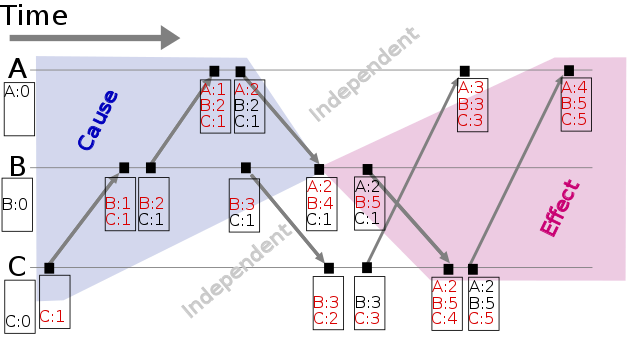
\includegraphics[width=11cm]{vector-clocks.png}
  {\small source \href{https://en.wikipedia.org/wiki/Vector_clock}{WikiPedia: Vector Clocks}}\\
  \end{center}
  Extension of Leslie Lamport's logical clocks.
\end{frame}

\begin{frame}[fragile]
  \frametitle{Execution Step}
  \framesubtitle{Vector Clocks}
  {\small
  \begin{minted}{haskell}
newtype VectorClock = VectorClock {
    getVectorClock :: Map IOSimThreadId Int
  }
leastUpperBoundVClock :: VectorClock
                      -> VectorClock
                      -> VectorClock
leastUpperBoundVClock (VectorClock m) (VectorClock m') =
    VectorClock (Map.unionWith max m m')
  \end{minted}
  }

  For example

  {\small
  \begin{minted}{haskell}
  ThrowTo e tid' k -> do
    let thread' = thread {
            threadEffect  = effect <> throwToEffect tid'
                                   <> wakeUpEffect,
            threadVClock  =
              vClock `leastUpperBoundVClock` vClockTgt
            ...
          }
        vClockTgt = threadVClock (threads Map.! tid')
  \end{minted}
  }

\end{frame}

\begin{frame}[fragile]
  \frametitle{IOSimPOR Schedule Policy}
  {\bf Run not blocked thread with the smallest \texttt{ThreadId}.}
  {\small
  \begin{minted}{haskell}
data IOSimThreadId =
    RacyThreadId [Int]
    -- | A non racy thread.  They have higher priority than
    -- racy threads in `IOSimPOR` scheduler.
  | ThreadId     [Int]
  \end{minted}

  \begin{minted}{haskell}
mainThread :: IOSimThreadId
mainThread = ThreadId []

-- second child of `RacyThread [1]`
threadId = RacyThreadId [1,2]
  \end{minted}
  }

As a consequence a thread will be scheduled until it is blocked.
\end{frame}

\begin{frame}[fragile]
  \frametitle{Races}
  \begin{onlyenv}<1->
  {\tiny
  \begin{minted}{haskell}
data StepInfo = StepInfo {
    -- | Step that we want to reschedule to run after a step in
    -- `stepInfoRaces`.
    stepInfoStep       :: Step,
    -- | Control information when we reach this step.
    stepInfoControl    :: ScheduleControl,
    -- | Threads that are still concurrent with this step.
    stepInfoConcurrent :: Set IOSimThreadId,
    -- | Steps following this one that did not happen after it
    -- (in reverse order).
    stepInfoNonDep     :: [Step],
    -- | Later steps that race with `stepInfoStep`.
    stepInfoRaces      :: [Step] }
  \end{minted}
  }
  \end{onlyenv}
  \vspace{1em}
  \begin{onlyenv}<2->
  {\small New schedules are constructed from \texttt{stepInfoRaces} and \texttt{stepInfoNonDep}:}
    \vspace{0.5em}
  {\tiny\begin{minted}{haskell}
    [    takeWhile (/=stepStepId racingStep)
                   (stepStepId <$> reverse stepInfoNonDep)
      ++ [stepStepId racingStep]
    | racingStep <- stepInfoRaces ]
  \end{minted}
  }
  \end{onlyenv}
%   {\small\begin{minted}{haskell}
% data Races = Races { -- These steps may race with future steps
%                      activeRaces   :: ![StepInfo],
%                      -- These steps cannot be concurrent with
%                      -- future steps
%                      completeRaces :: ![StepInfo] }
%   \end{minted}
%   }
\end{frame}

\begin{frame}[fragile]
  \frametitle{Races}
  \framesubtitle{Recording new StepInfo in active races}

  {\small
  \begin{minted}{haskell}
-- A new step to add to the `activeRaces` list.
newStepInfo :: Maybe StepInfo
newStepInfo | isNotRacyThreadId tid = Nothing
            | Set.null concurrent   = Nothing
            | isBlocking            = Nothing
            | otherwise =
    Just StepInfo { stepInfoStep       = newStep,
                    stepInfoControl    = control,
                    stepInfoConcurrent = concurrent,
                    stepInfoNonDep     = [],
                    stepInfoRaces      = []
                  }
  where
    concurrent :: Set IOSimThreadId
    concurrent = concurrent0 Set.\\ effectWakeup newEffect
    isBlocking :: Bool
    isBlocking = isThreadBlocked thread
              && onlyReadEffect newEffect
  \end{minted}
  % concurrent0 = 
  %   Map.keysSet (Map.filter (\t -> not (isThreadDone t)
  %                               && threadId t `Set.notMember`
  %                                  effectForks (stepEffect newStep)
  %                           ) threads)
  }
\end{frame}

\begin{frame}[fragile]
  \frametitle{Races}
  \framesubtitle{Updating already recorded active races}
  With every new step, we need to update existing information recorded in \texttt{StepInfo}.
  {\tiny
  \begin{minted}{haskell}
     let theseStepsRace = step `racingSteps` newStep
         -- `step` happened before `newStep` (`newStep` happened after
         -- `step`)
         happensBefore   = step `happensBeforeStep` newStep
         -- `newStep` happens after any of the racing steps
         afterRacingStep = any (`happensBeforeStep` newStep) stepInfoRaces
  \end{minted}
  }
  \begin{itemize}
    \item<2-> update \texttt{stepInfoConcurrent}
      \begin{onlyenv}<2>
      \tiny
      \begin{minted}{haskell}
         let -- We will only record the first race with each thread.
             -- Reversing the first race makes the next race detectable.
             -- Thus we remove a thread from the concurrent set after the
             -- first race.
             concurrent'
               | happensBefore   = Set.delete tid concurrent
                            Set.\\ effectWakeup newEffect
               | theseStepsRace  = Set.delete tid concurrent
               | afterRacingStep = Set.delete tid concurrent
               | otherwise       = concurrent
      \end{minted}
      \end{onlyenv}
    \item<3-> update \texttt{stepInfoNonDep}
      \begin{onlyenv}<3>
      \tiny
      \begin{minted}{haskell}
         let stepInfoNonDep'
               -- `newStep` happened after `step`
               | happensBefore =           stepInfoNonDep
               -- `newStep` did not happen after `step`
               | otherwise     = newStep : stepInfoNonDep
      \end{minted}
      \end{onlyenv}
    \item<4-> update \texttt{stepInfoRaces}
      \begin{onlyenv}<4>
      \tiny
      \begin{minted}{haskell}
         let -- Here we record discovered races.  We only record new
             -- race if we are following the default schedule, to avoid
             -- finding the same race in different parts of the search
             -- space.
             stepInfoRaces'
               | theseStepsRace && isDefaultSchedule control
                           = newStep : stepInfoRaces
               | otherwise =           stepInfoRaces
      \end{minted}
      \end{onlyenv}
  \end{itemize}
\end{frame}

\begin{frame}[fragile]
  \frametitle{Example}
  \begin{minted}{haskell}
sim :: IOSim s ()
sim = do
  exploreRaces
  v <- newTVarIO False
  forkIO (atomically $ writeTVar v True)
  forkIO (readTVarIO v >>= say . show)
  -- wait for both threads to terminate.
  threadDelay 1_000_000

quickCheck $ exploreSimTrace
      (\a -> a { explorationDebugLevel = 1 })
      sim
      (\_ _ -> True)
  \end{minted}
\end{frame}

\begin{frame}[fragile]
  \frametitle{Example: default schedule}
  \begin{columns}
    \begin{column}{0.4\textwidth}
      \begin{figure}[t]
        \begin{flushleft}
        \begin{tcolorbox}
        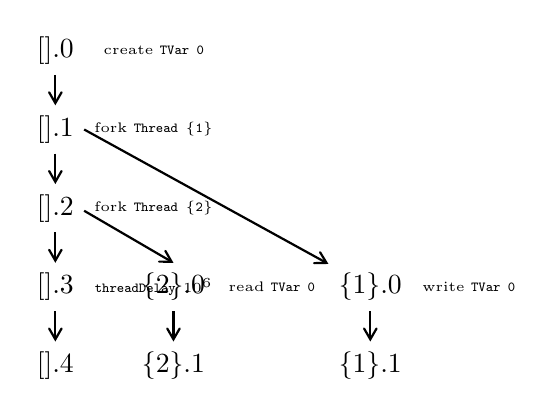
\begin{tikzpicture}
          \draw <1-> node (A0)  at (0, 0) {[].0};
          \draw <1-> node (A0') at (1.25, 0) {\tiny create \texttt{TVar 0}};
          \draw <2-> node (A1)  at (0,-1) {[].1};
          \draw <2>  node (A1') at (1.25, -1) {\tiny fork \texttt{Thread \{1\}}};
          \draw <3-> node (A2)  at (0,-2) {[].2};
          \draw <3>  node (A2') at (1.25,-2) {\tiny fork \texttt{Thread \{2\}}};
          \draw <4-> node (A3)  at (0,-3) {[].3};
          \draw <4>  node (A3') at (1.25,-3) {\tiny \texttt{threadDelay $10^6$}};
          \draw <10-> node (A4)  at (0,-4) {[].4};

          \draw <7-> node (B0)  at (4.0,-3) {\{1\}.0};
          \draw <7-> node (B0') at (5.25,-3) {\tiny write \texttt{TVar 0}};
          \draw <8-> node (B1)  at (4.0,-4) {\{1\}.1};

          \draw <5-> node (C0)  at (1.5,-3) {\{2\}.0};
          \draw <5-> node (C0') at (2.75,-3) {\tiny read \texttt{TVar 0}};
          \draw <6-> node (C1)  at (1.5,-4) {\{2\}.1};

          \draw <2-> [->] (A0) -- (A1);
          \draw <3-> [->] (A1) -- (A2);
          \draw <4-> [->] (A2) -- (A3);
          \draw <10-> [->] (A3) -- (A4);
          \draw <7-> [->] (A1.0) -- (B0);
          \draw <8-> [->] (B0) -- (B1);
          \draw <5-> [->] (A2.355) -- (C0.90);
          \draw <6-> [->] (C0) -- (C1);
        \end{tikzpicture}
        \end{tcolorbox}
        \end{flushleft}
      \end{figure}
    \end{column}

    \begin{column}{0.6\textwidth}
      \begin{onlyenv}<1>
        \tiny
        \begin{verbatim}
0s - Thread [].0 main - SimStart ControlDefault
0s - Thread [].0 main - TxCommitted [] [TVarId 0] Effect {  }
0s - Thread [].0 main - Unblocked []
0s - Thread [].0 main - Deschedule Yield
0s - Thread [].0 main - Effect VectorClock [Thread [].0]
                               Effect {  }
        \end{verbatim}
      \end{onlyenv}
      \begin{onlyenv}<2>
        \tiny
        \begin{verbatim}
0s - Thread [].1 main - ThreadForked Thread {1}
0s - Thread [].1 main - Deschedule Yield
0s - Thread [].1 main - Effect VectorClock [Thread [].1]
                               Effect { forks = [Thread {1}] }
        \end{verbatim}
      \end{onlyenv}
      \begin{onlyenv}<3>
        \tiny
        \begin{verbatim}
0s - Thread [].2 main - ThreadForked Thread {2}
0s - Thread [].2 main - Deschedule Yield
0s - Thread [].2 main - Effect VectorClock [Thread [].2]
                               Effect { forks = [Thread {2}] }
        \end{verbatim}
      \end{onlyenv}
      \begin{onlyenv}<4>
        \tiny
        \begin{verbatim}
0s - Thread [].3 main - ThreadDelay TimeoutId 0 Time 1s
0s - Thread [].3 main - Effect VectorClock [Thread [].3]
                               Effect {  }
        \end{verbatim}
      \end{onlyenv}
      \begin{onlyenv}<5>
        \tiny
        \begin{minted}{haskell}
data StepInfo = StepInfo {
    stepInfoStep       = Step ({2}.0),
    stepInfoControl    = DefaultControl,
    stepInfoConcurrent = Set.fromList
                         [[], {1}, {2}],
    stepInfoNonDep     = [],
    stepInfoRaces      = []
  }

        \end{minted}
        \begin{verbatim}
0s - Thread {2}.0  - TxCommitted [] []
                       Effect { reads = fromList [TVarId 0] }
0s - Thread {2}.0  - Unblocked []
0s - Thread {2}.0  - Deschedule Yield
0s - Thread {2}.0  - Effect VectorClock [Thread {2}.0,
                                         Thread [].2]
                       Effect { reads = fromList [TVarId 0] }
        \end{verbatim}
      \end{onlyenv}
      \begin{onlyenv}<6>
        \tiny
        \begin{minted}{haskell}
data StepInfo = StepInfo {
    stepInfoStep       = Step ({2}.0),
    stepInfoControl    = DefaultControl,
    stepInfoConcurrent = Set.fromList
                         [[], {1}],
    stepInfoNonDep     = [],
    stepInfoRaces      = []
  }

        \end{minted}
        \begin{verbatim}
0s - Thread {2}.1  - Say False
0s - Thread {2}.1  - ThreadFinished
0s - Thread {2}.1  - Deschedule Terminated
0s - Thread {2}.1  - Effect VectorClock [Thread {2}.1,
                                         Thread [].2]
                      Effect {  }
        \end{verbatim}
      \end{onlyenv}
      \begin{onlyenv}<7>
        \tiny
        \begin{minted}{haskell}
data StepInfo = StepInfo {
    stepInfoStep       = Step ({2}.0),
    stepInfoControl    = DefaultControl,
    stepInfoConcurrent = Set.fromList
                         [[], {1}],
    stepInfoNonDep     = [{1}.0],
    stepInfoRaces      = [{1}.0]
  }

        \end{minted}
        \begin{verbatim}
0s - Thread {1}.0  - TxCommitted [TVarId 0] []
                      Effect { writes = fromList [TVarId 0] }
0s - Thread {1}.0  - Unblocked []
0s - Thread {1}.0  - Deschedule Yield
0s - Thread {1}.0  - Effect VectorClock [Thread {1}.0,
                                         Thread [].1]
                      Effect { writes = fromList [TVarId 0] }
        \end{verbatim}
      \end{onlyenv}
      \begin{onlyenv}<8>
        \tiny
        \begin{minted}{haskell}
data StepInfo = StepInfo {
    stepInfoStep       = Step ({2}.0),
    stepInfoControl    = DefaultControl,
    stepInfoConcurrent = Set.fromList
                         [[]],
    stepInfoNonDep     = [{1}.0],
    stepInfoRaces      = [{1}.0]
  }

        \end{minted}
        \begin{verbatim}
0s - Thread {1}.1  - ThreadFinished
0s - Thread {1}.1  - Deschedule Terminated
0s - Thread {1}.1  - Effect VectorClock [Thread {1}.1,
                                         Thread [].1]
                            Effect {  }
RacesFound [ControlAwait [ScheduleMod (RacyThreadId [2],0)
                                      ControlDefault
                                      [(RacyThreadId [1],0)]]]
        \end{verbatim}
      \end{onlyenv}
      \begin{onlyenv}<9>
        \tiny
        \begin{minted}{haskell}
data StepInfo = StepInfo {
    stepInfoStep       = Step ({2}.0),
    stepInfoControl    = DefaultControl,
    stepInfoConcurrent = Set.fromList
                         [[]],
    stepInfoNonDep     = [{1}.0],
    stepInfoRaces      = [{1}.0]
  }

        \end{minted}
        \begin{verbatim}
1s - Thread [].- thread delay timer - ThreadDelayFired
                                        TimeoutId 0
        \end{verbatim}
      \end{onlyenv}
      \begin{onlyenv}<10->
        \tiny
        \begin{minted}{haskell}
data StepInfo = StepInfo {
    stepInfoStep       = Step ({2}.0),
    stepInfoControl    = DefaultControl,
    stepInfoConcurrent = Set.fromList
                         [[]],
    stepInfoNonDep     = [{1}.0],
    stepInfoRaces      = [{1}.0]
  }

        \end{minted}
        \begin{verbatim}
1s - Thread [].4 main - ThreadFinished
1s - Thread [] main - MainReturn () []
        \end{verbatim}
      \end{onlyenv}
    \end{column}
  \end{columns}
\end{frame}

\begin{frame}[fragile]
  \frametitle{Example: discovered schedule}
  \begin{columns}
    \begin{column}{0.4\textwidth}
      \begin{figure}
        \begin{tcolorbox}
          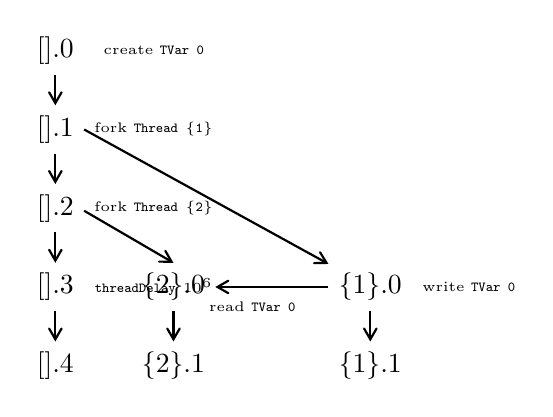
\begin{tikzpicture}
            \draw <1-> node (A0)  at (0, 0) {[].0};
            \draw <1-> node (A0') at (1.25, 0) {\tiny create \texttt{TVar 0}};
            \draw <2-> node (A1)  at (0,-1) {[].1};
            \draw <2>  node (A1') at (1.25, -1) {\tiny fork \texttt{Thread \{1\}}};
            \draw <3-> node (A2)  at (0,-2) {[].2};
            \draw <3>  node (A2') at (1.25,-2) {\tiny fork \texttt{Thread \{2\}}};
            \draw <4-> node (A3)  at (0,-3) {[].3};
            \draw <4>  node (A3') at (1.25,-3) {\tiny \texttt{threadDelay $10^6$}};
            \draw <11-> node (A4)  at (0,-4) {[].4};

            \draw <6-> node (B0)  at (4.0,-3) {\{1\}.0};
            \draw <6-> node (B0') at (5.25,-3) {\tiny write \texttt{TVar 0}};
            \draw <9-> node (B1)  at (4.0,-4) {\{1\}.1};

            \draw <7-> node (C0)  at (1.5,-3) {\{2\}.0};
            \draw <7-> node (C0') at (2.5,-3.25) {\tiny read \texttt{TVar 0}};
            \draw <8-> node (C1)  at (1.5,-4) {\{2\}.1};

            \draw <2-> [->] (A0) -- (A1);
            \draw <3-> [->] (A1) -- (A2);
            \draw <4-> [->] (A2) -- (A3);
            \draw <11-> [->] (A3) -- (A4);
            \draw <6-> [->] (A1.0) -- (B0);
            \draw <9-> [->] (B0) -- (B1);
            \draw <7-> [->] (A2.355) -- (C0.90);
            \draw <7-> [->] (B0) -- (C0);
            \draw <8-> [->] (C0) -- (C1);
          \end{tikzpicture}
        \end{tcolorbox}
      \end{figure}
    \end{column}

    \begin{column}{0.6\textwidth}
      \tiny
      \begin{onlyenv}<1>
        \begin{verbatim}
0s - Thread [].0 main - SimStart ControlAwait
                            [ScheduleMod (RacyThreadId [2],0)
                                         ControlDefault
                                         [(RacyThreadId [1],0)]]
0s - Thread [].0 main - TxCommitted [] [TVarId 0] Effect {  }
0s - Thread [].0 main - Unblocked []
0s - Thread [].0 main - Deschedule Yield
0s - Thread [].0 main - Effect VectorClock [Thread [].0]
                          Effect {  }
        \end{verbatim}
      \end{onlyenv}
      \begin{onlyenv}<2>
        \begin{verbatim}
0s - Thread [].1 main - ThreadForked Thread {1}
0s - Thread [].1 main - Deschedule Yield
0s - Thread [].1 main - Effect VectorClock [Thread [].1]
                          Effect { forks = [Thread {1}] }
        \end{verbatim}
      \end{onlyenv}
      \begin{onlyenv}<3>
        \begin{verbatim}
0s - Thread [].2 main - ThreadForked Thread {2}
0s - Thread [].2 main - Deschedule Yield
0s - Thread [].2 main - Effect VectorClock [Thread [].2]
                          Effect { forks = [Thread {2}] }
        \end{verbatim}
      \end{onlyenv}
      \begin{onlyenv}<4>
        \begin{verbatim}
0s - Thread [].3 main - ThreadDelay TimeoutId 0 Time 1s
0s - Thread [].3 main - Effect VectorClock [Thread [].3]
                          Effect {  }
        \end{verbatim}
      \end{onlyenv}
      \begin{onlyenv}<5>
        \begin{verbatim}
0s - Thread {2}.0  - FollowControl ControlAwait
                      [ScheduleMod (RacyThreadId [2],0)
                                   ControlDefault
                                   [(RacyThreadId [1],0)]]
0s - Thread {2}.0  - AwaitControl Thread {2}.0 ControlFollow [(RacyThreadId [1],0)] []
0s - Thread {2}.0  - Deschedule Sleep
        \end{verbatim}
      \end{onlyenv}
      \begin{onlyenv}<6>
        \begin{verbatim}
0s - Thread {1}.0  - Reschedule ControlFollow
                                [(RacyThreadId [1],0)] []
0s - Thread {1}.0  - PerformAction Thread {1}.0
0s - Thread {1}.0  - TxCommitted [TVarId 0] []
                      Effect { writes = fromList [TVarId 0] }
0s - Thread {1}.0  - Unblocked []
0s - Thread {1}.0  - Deschedule Yield
0s - Thread {1}.0  - Effect
                      VectorClock [Thread {1}.0,
                                   Thread [].1]
                      Effect { writes = fromList [TVarId 0] }
        \end{verbatim}
      \end{onlyenv}
      \begin{onlyenv}<7>
        \begin{verbatim}
0s - Thread {2}.0  - TxCommitted [] []
                       Effect { reads = fromList [TVarId 0] }
0s - Thread {2}.0  - Unblocked []
0s - Thread {2}.0  - Deschedule Yield
0s - Thread {2}.0  - Effect
                      VectorClock [Thread {1}.0,
                                   Thread {2}.0,
                                   Thread [].2]
                      Effect { reads = fromList [TVarId 0] }
        \end{verbatim}
      \end{onlyenv}
      \begin{onlyenv}<8>
        \begin{verbatim}
0s - Thread {2}.1  - Say True
0s - Thread {2}.1  - ThreadFinished
0s - Thread {2}.1  - Deschedule Terminated
0s - Thread {2}.1  - Effect
                       VectorClock [Thread {1}.0,
                                    Thread {2}.1,
                                    Thread [].2]
                       Effect {  }
        \end{verbatim}
      \end{onlyenv}
      \begin{onlyenv}<9>
        \begin{verbatim}
0s - Thread {1}.1  - ThreadFinished
0s - Thread {1}.1  - Deschedule Terminated
0s - Thread {1}.1  - Effect
                      VectorClock [Thread {1}.1,
                                   Thread [].1]
                      Effect {  }
RacesFound [ControlAwait
              [ScheduleMod (RacyThreadId [2],0)
                           ControlDefault
                           [(RacyThreadId [1],0)]]]
        \end{verbatim}
      \end{onlyenv}
      \begin{onlyenv}<10>
        \begin{verbatim}
1s - Thread [].- thread delay timer -
                    ThreadDelayFired TimeoutId 0
        \end{verbatim}
      \end{onlyenv}
      \begin{onlyenv}<11->
        \begin{verbatim}
1s - Thread [].4 main - ThreadFinished
RacesFound []
1s - Thread [] main - MainReturn () []
        \end{verbatim}
      \end{onlyenv}
    \end{column}
  \end{columns}
\end{frame}

\begin{frame}[fragile]
  \frametitle{Example 2}
  {\small\begin{minted}{haskell}
sim :: IOSim s ()
sim = do
  exploreRaces
  v0 <- newTVarIO False
  v1 <- newTVarIO False
  forkIO (do atomically (writeTVar v0 True) -- Thread {1}.0
             atomically (readTVar  v1)      -- Thread {1}.1
               >>= say . show . ("v1",))
  forkIO (do atomically (writeTVar v1 True) -- Thread {2}.0
             atomically (readTVar  v0)      -- Thread {2}.1
               >>= say . show . ("v0",))
  -- wait for both threads to terminate.
  threadDelay 1_000_000
  \end{minted}
  }
\end{frame}

\begin{frame}[fragile]
  \frametitle{Example 2}
  Three schedules:

  {\small\begin{itemize}
    \item<2-> \mint{haskell}|ControlDefault|
              \begin{itemize}
                \item[] \mint{haskell}|("v0", False)|
                \item[] \mint{haskell}|("v1", True)|
              \end{itemize}
    \item<3-> \begin{minted}{haskell}
ScheduleMod (RacyThreadId [2],1) ControlDefault
            [(RacyThreadId [1],0)]]
              \end{minted}
              \begin{itemize}
                \item[] \mint{haskell}|("v0", True)|
                \item[] \mint{haskell}|("v1", True)|
              \end{itemize}
    \item<4-> \begin{minted}{haskell}
ScheduleMod (RacyThreadId [2],0) ControlDefault
            [(RacyThreadId [1],0),(RacyThreadId [1],1)]
              \end{minted}
              \begin{itemize}
                \item[] \mint{haskell}|("v0", True)|
                \item[] \mint{haskell}|("v1", False)|
              \end{itemize}
    \end{itemize}}
\end{frame}

\begin{frame}
  \vspace{10em}
  \begin{center}
  {\huge Fair winds and following seas, me mateys!}\\
  \end{center}
  \vspace{2em}
  \begin{flushright}
    
\includegraphics[width=2cm]{coot.me.png}\\
    \url{https://coot.me}
  \end{flushright}
\end{frame}

\end{document}

